\suppressfloats[t]
\section{Experimental Configuration}
\label{app:configuration}

\paragraph{Environment and learner.}
The primary environment is the six-node \texttt{NetworkManagement-v1} inventory network. Node 1 is
scripted; nodes 2--6 are controlled by one parameter-shared PPO policy. The padded joint observation
is visible to the actor, while each vector lane supplies the action for one trainable node. Unless a
specific experiment states otherwise, PPO uses the Stable-Baselines3 defaults with
\texttt{n\_steps}$=128$, minibatch size 256, ten optimization epochs, learning rate
$3\times10^{-4}$, discount $.99$, GAE coefficient $.95$, policy clip $.2$, value-loss coefficient
$.5$, zero entropy coefficient, normalized minibatch advantages, and global gradient max-norm $.5$.
Training is CPU-only and uses a single explicit simulator random stream per environment.

\paragraph{Reward and label.}
Each agent receives $x_i(w)=(1-w)r_i^{\mathrm{local}}+wr^{\mathrm{global}}$ before any transform.
The supply-chain collapse label is
$\mathbf{1}[\bar S<10\wedge\bar\pi\le-127.1]$, where $\bar S$ is the mean deterministic base-stock
action across the five trained nodes and $\bar\pi$ is their ten-episode mean total profit. The label
is evaluated independently of the transformed training reward. Its profit clause is a redundancy
check because collapsed policies concentrate at the deterministic lazy-policy floor near $-128$.
Evaluation seed blocks are $10s,\ldots,10s+9$ for training seed $s$.

\paragraph{Transform conditions.}
The linear condition uses $v(x)=x$. Curvature-only uses
$\phi(x)=\operatorname{sign}(x)|x|^{.88}$. The loss-multiplier condition uses
$v_\lambda(x)=\phi(x)$ for $x\ge0$ and $\lambda\phi(x)$ for $x<0$. The independent direct control
uses the fixed reference $z_0=-2.6281398333$, estimated before confirmation from 60,000 equally
weighted blend samples produced by 40 untreated calibration policies. With $u=x-z_0$, its arms are
$B=\phi(u)$, $A=v_7(u)$, and $S=7\phi(u)$.

\section{Boundary Estimation and Diagnostics}
\label{app:estimation}

For each fixed configuration we fit
$P(Y=1\mid w)=\sigma(b_0+b_1w)$ by Firth logistic regression and report
$w_{50}=-b_0/b_1$. A point estimate is reported only with a nonzero identified slope; observed
probabilities are inspected separately for adjacent cells bracketing $.5$. Confidence intervals use
2,000 percentile-bootstrap draws of complete training-seed blocks. The same multiplicity vector is
used across conditions in paired contrasts. Fits outside $[0,1]$ and nonconverged or unidentified
draws are retained and counted rather than clipped or silently replaced.

Logistic, probit, and decreasing isotonic fits are sensitivity estimators. The primary supply-PPO
point-estimator spread is at most .018. The independent confirmation was also reproduced with a
separate numerical optimizer to within $4\times10^{-9}$ at all fifteen primary budget/condition
points. Confidence intervals are pointwise; no simultaneous statement across checkpoints is made.

\begin{table*}[t]
\caption{Observed supply PPO collapse counts at 300k. Entries are $w:k/n$; Wilson intervals and all-setting cell records are exported in collapse\_cells.csv.}
\label{tab:observed_cells}
\centering\small
\begin{tabular}{@{}lp{0.84\textwidth}@{}}
\toprule
Condition & Observed cells \\
\midrule
null & 0.00: 20/20, 0.20: 20/20, 0.40: 20/20, 0.50: 20/20, 0.60: 17/20, 0.70: 10/20, 0.80: 0/20, 0.90: 0/20, 1.00: 0/20 \\
$\lambda=$1 & 0.50: 17/20, 0.65: 3/20, 0.75: 2/20, 0.85: 1/20, 0.95: 0/20 \\
$\lambda=$2 & 0.50: 20/20, 0.65: 17/20, 0.75: 6/20, 0.85: 0/20, 0.95: 0/20 \\
$\lambda=$3 & 0.50: 20/20, 0.65: 19/20, 0.75: 15/20, 0.85: 1/20, 0.95: 0/20 \\
$\lambda=$4 & 0.50: 20/20, 0.65: 20/20, 0.75: 18/20, 0.85: 3/20, 0.95: 0/20 \\
$\lambda=$5 & 0.50: 20/20, 0.65: 20/20, 0.75: 20/20, 0.80: 17/20, 0.85: 3/20, 0.90: 0/20, 0.95: 0/20 \\
$\lambda=$6 & 0.50: 20/20, 0.65: 20/20, 0.75: 17/20, 0.80: 17/20, 0.85: 10/20, 0.90: 0/20, 0.95: 0/20 \\
$\lambda=$7 & 0.50: 20/20, 0.65: 20/20, 0.75: 20/20, 0.80: 19/20, 0.85: 11/20, 0.90: 1/20, 0.95: 0/20 \\
\bottomrule
\end{tabular}
\end{table*}

\begin{table}[t]
\caption{Full supply PPO sweep after inclusion of all 120 completed refinement runs. Slopes are Firth estimates; no legacy Wald significance claims are retained.}
\label{tab:lambda_sweep}
\centering\small
\begin{tabular}{@{}rrlrr@{}}
\toprule
$\lambda$ & Runs & Midpoint and 95\% CI & Slope & Usable \\
\midrule
1 & 100 & $0.585$ $[0.544,0.624]$ & $-14.72$ & 2000/2000 \\
2 & 100 & $0.714$ $[0.683,0.745]$ & $-27.24$ & 2000/2000 \\
3 & 100 & $0.775$ $[0.755,0.790]$ & $-29.68$ & 2000/2000 \\
4 & 100 & $0.805$ $[0.780,0.829]$ & $-36.84$ & 2000/2000 \\
5 & 140 & $0.825$ $[0.812,0.838]$ & $-67.01$ & 2000/2000 \\
6 & 140 & $0.835$ $[0.816,0.853]$ & $-33.55$ & 2000/2000 \\
7 & 140 & $0.852$ $[0.840,0.865]$ & $-55.23$ & 2000/2000 \\
\bottomrule
\end{tabular}
\end{table}

\FloatBarrier

\section{Independent Longitudinal Confirmation}
\label{app:confirmation}

Pilot seeds 100--104 selected a common five-cell grid. The subsequent confirmation was frozen before
execution and uses disjoint seeds 42--51, three reward conditions, and
$w\in\{.2,.4,.6,.85,1\}$. All 150 trajectories start from initialization, run to 3.6M requested
agent transitions, and are evaluated every 150k transitions. Pilot outcomes do not enter the
confirmation estimates. Every scheduled evaluation, configuration, transition counter, evaluation
seed, source hash, and collapse label was checked before analysis.

\begin{table*}[t]
\centering\small
\caption{Independent confirmation: ten seeds per condition and cell; 2,000 paired seed-block bootstrap draws. $\dagger$ marks identical seed-label patterns and zero bootstrap width; the empirical bracket remains $[.6,.85]$. Intervals are pointwise.}
\label{tab:confirmed_horizon}
\begin{tabular}{@{}rllll@{}}\toprule
Budget & Linear & Curvature & Loss multiplier 7 & Multiplier minus curvature \\
\midrule
300k & $0.648$ $[0.582,0.725]$ & $0.562$ $[0.500,0.626]$ & $0.843$ $[0.778,0.893]$ & $0.281$ $[0.174,0.363]$ \\
900k & $0.543$ $[0.500,0.604]$ & $0.441$ $[0.332,0.543]$ & $0.725$ $[0.725,0.725]$$^{\dagger}$ & $0.284$ $[0.182,0.393]$ \\
1800k & $0.589$ $[0.500,0.698]$ & $0.399$ $[0.291,0.503]$ & $0.725$ $[0.725,0.725]$$^{\dagger}$ & $0.326$ $[0.222,0.433]$ \\
3600k & $0.590$ $[0.482,0.700]$ & $0.524$ $[0.420,0.630]$ & $0.670$ $[0.604,0.725]$ & $0.146$ $[0.072,0.229]$ \\
\bottomrule\end{tabular}
\end{table*}

\begin{table*}[t]
\centering\small
\caption{Observed collapsed/total counts for the independent horizon confirmation at the four primary budgets. The same ten seeds occur at every cell and budget. All 24 checkpoint panels remain in the raw exports.}
\label{tab:confirmed_cells}
\begin{tabular}{@{}rlrrrrr@{}}\toprule
Budget & Condition & $w=.2$ & $.4$ & $.6$ & $.85$ & $1$ \\
\midrule
300k & Linear & 10/10 & 10/10 & 7/10 & 0/10 & 0/10 \\
300k & Curvature only & 10/10 & 10/10 & 3/10 & 0/10 & 0/10 \\
300k & Loss multiplier 7 & 10/10 & 10/10 & 10/10 & 5/10 & 0/10 \\
900k & Linear & 10/10 & 10/10 & 2/10 & 0/10 & 0/10 \\
900k & Curvature only & 9/10 & 7/10 & 1/10 & 0/10 & 0/10 \\
900k & Loss multiplier 7 & 10/10 & 10/10 & 10/10 & 0/10 & 0/10 \\
1800k & Linear & 10/10 & 10/10 & 2/10 & 1/10 & 1/10 \\
1800k & Curvature only & 9/10 & 5/10 & 1/10 & 0/10 & 0/10 \\
1800k & Loss multiplier 7 & 10/10 & 10/10 & 10/10 & 0/10 & 0/10 \\
3600k & Linear & 10/10 & 9/10 & 2/10 & 3/10 & 0/10 \\
3600k & Curvature only & 10/10 & 7/10 & 4/10 & 0/10 & 0/10 \\
3600k & Loss multiplier 7 & 10/10 & 10/10 & 8/10 & 0/10 & 0/10 \\
\bottomrule\end{tabular}
\end{table*}


\begin{figure}[t]
\centering
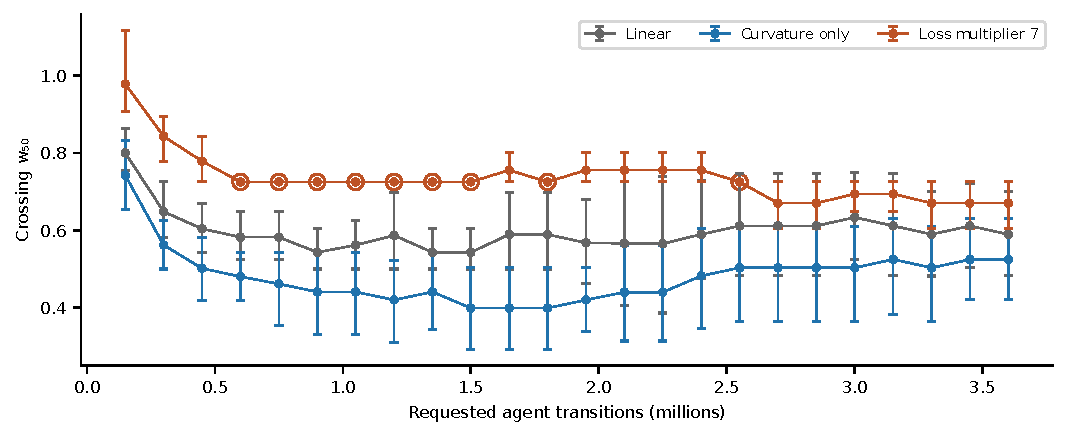
\includegraphics[width=.92\textwidth]{generated/confirmation/horizon_all_checkpoints.pdf}
\caption{All independent-confirmation checkpoints with untruncated pointwise seed-block intervals.
Open rings mark zero-width bootstrap intervals caused by identical seed-label patterns on the coarse
grid; they do not imply exact localization.}
\label{fig:confirmed_checkpoints}
\end{figure}

\subsection{Recovery, relapse, and evaluation sensitivity}

Recovery and relapse are descriptive within-policy outcomes conditional on the 300k label. Sustained
recovery is the first occurrence of three consecutive noncollapsed checkpoints after 300k and may be
followed by relapse. These proportions describe the five fixed mixture cells rather than a task-level
population distribution.

\begin{table*}[t]
\centering\small
\caption{Within-policy outcomes conditional on the 300k label, by mixture cell. Recovery/relapse columns describe the 3.6M state. Sustained recovery means ever observing three consecutive noncollapsed checkpoints after 300k; it need not persist to 3.6M. A dash denotes a zero denominator.}
\label{tab:confirmed_recovery}
\begin{tabular}{@{}lrrrrr@{}}\toprule
Condition & $w$ & Collapsed at 300k & Recovered at 3.6M & Ever sustained & Relapsed at 3.6M \\
\midrule
Linear & 0.2 & 10 & 0/10 & 1/10 & -- \\
Linear & 0.4 & 10 & 1/10 & 1/10 & -- \\
Linear & 0.6 & 7 & 5/7 & 5/7 & 0/3 \\
Linear & 0.85 & 0 & -- & -- & 3/10 \\
Linear & 1 & 0 & -- & -- & 0/10 \\
Curvature only & 0.2 & 10 & 0/10 & 1/10 & -- \\
Curvature only & 0.4 & 10 & 3/10 & 5/10 & -- \\
Curvature only & 0.6 & 3 & 1/3 & 2/3 & 2/7 \\
Curvature only & 0.85 & 0 & -- & -- & 0/10 \\
Curvature only & 1 & 0 & -- & -- & 0/10 \\
Loss multiplier 7 & 0.2 & 10 & 0/10 & 0/10 & -- \\
Loss multiplier 7 & 0.4 & 10 & 0/10 & 0/10 & -- \\
Loss multiplier 7 & 0.6 & 10 & 2/10 & 2/10 & -- \\
Loss multiplier 7 & 0.85 & 5 & 5/5 & 5/5 & 0/5 \\
Loss multiplier 7 & 1 & 0 & -- & -- & 0/10 \\
\bottomrule\end{tabular}
\end{table*}


\begin{figure}[t]
\centering
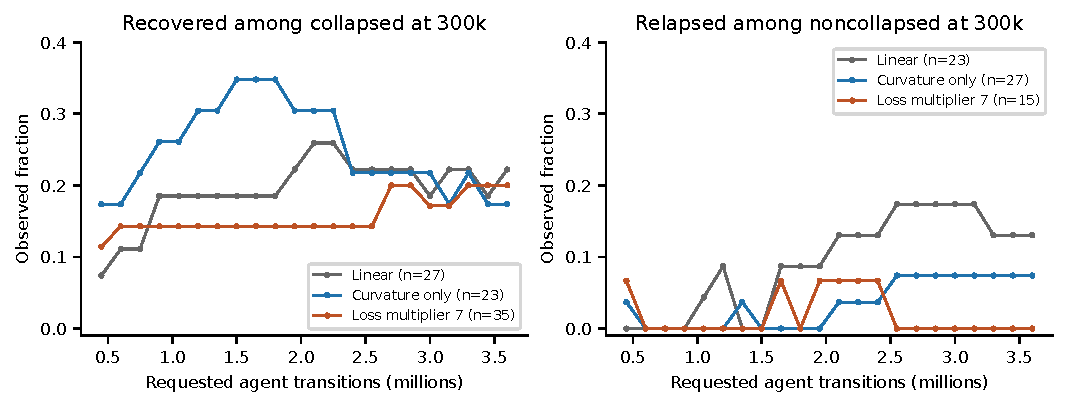
\includegraphics[width=.9\textwidth]{generated/confirmation/recovery_trajectories.pdf}
\caption{Observed recovery and relapse fractions conditional on the 300k label. Curves show current
checkpoint state and do not establish an absorbing transition or convergence.}
\label{fig:confirmed_recovery}
\end{figure}

The fifty-episode sensitivity evaluation shares its first ten episodes with the primary evaluation and
preserves training random state. Only one of 450 trajectory/checkpoint labels changes; the 1.8M and
3.6M contrasts are unchanged.

\begin{table*}[t]
\centering\small
\caption{Loss-multiplier-minus-curvature contrast under ten versus fifty evaluation episodes. Only one of 450 trajectory/checkpoint labels changes (curvature, $w=.4$, seed 51, 900k). The fifty episodes include the original ten and are a sensitivity check, not an independent replication.}
\label{tab:confirmed_eval}
\begin{tabular}{@{}rll@{}}\toprule
Budget & Ten episodes & Fifty episodes \\
\midrule
900k & $0.284$ $[0.182,0.393]$ & $0.305$ $[0.204,0.414]$ \\
1800k & $0.326$ $[0.222,0.433]$ & $0.326$ $[0.222,0.433]$ \\
3600k & $0.146$ $[0.072,0.229]$ & $0.146$ $[0.072,0.229]$ \\
\bottomrule\end{tabular}
\end{table*}

\FloatBarrier

\section{Direct Asymmetric-versus-Symmetric Control}
\label{app:direct_control}

The control cohort contains $3\times8\times10=240$ independently trained policies at 300k requested
transitions. All arms use the same empirical-mean reference, mixture cells, training seeds, evaluation
seeds, learner, and optimizer. Four of 2,000 symmetric-arm bootstrap crossings fall outside the
sampled grid and remain in the interval calculation.

\begin{table*}[t]
\centering\small
\caption{Direct control at 300k with common empirical-mean reference, eight mixture cells and ten seeds; Firth fits with 2,000 seed-block draws.}
\label{tab:confirmed_control}
\begin{tabular}{@{}lll@{}}\toprule
Arm & Transform & Crossing and 95\% interval \\
\midrule
B & $\phi(u)$ & $0.560$ $[0.516,0.600]$ \\
A & $v_7(u)$ & $0.821$ $[0.775,0.864]$ \\
S & $7\phi(u)$ & $0.883$ $[0.821,0.954]$ \\
\bottomrule\end{tabular}
\end{table*}


\begin{figure}[t]
\centering
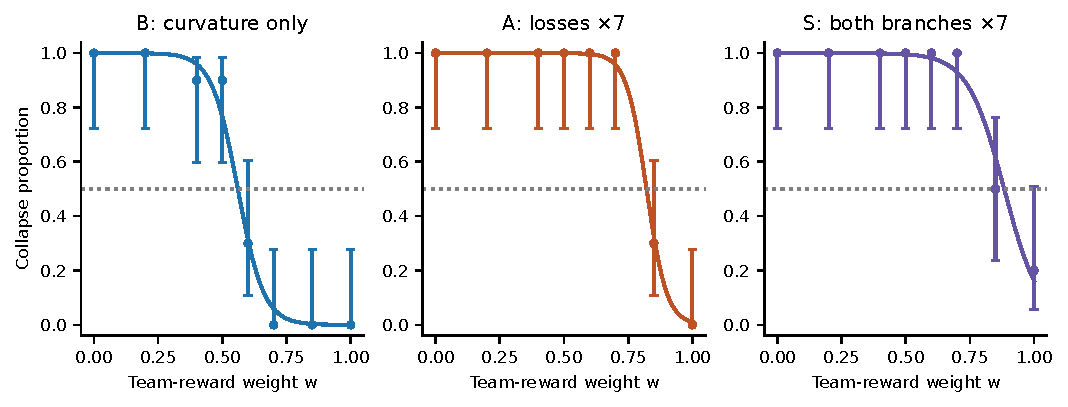
\includegraphics[width=.95\textwidth]{generated/confirmation/control_observations.pdf}
\caption{Observed collapse proportions for the three direct-control arms. Each point represents ten
training seeds; bars are 95\% Wilson intervals and curves are Firth fits over the sampled grid.}
\label{fig:confirmed_controls}
\end{figure}

The paired differences are $A-B=+.261$ $[.203,.329]$, $S-B=+.323$ $[.241,.427]$, and
$A-S=-.062$ $[-.157,.028]$. Thus both multipliers shift the crossing, whereas their direct difference
establishes neither an asymmetry-specific effect nor practical equivalence.

Near the empirical crossing brackets, loss fractions are 33.966\%, 31.096\%, and 20.393\% for B, A,
and S. Across all cells, transformed-reward RMS values are 8.796, 30.359, and 57.673; raw rollout
advantage standard deviations are 35.045, 135.948, and 300.400. Normalized optimizer-advantage
standard deviation is .997653 in every arm. Nevertheless, every control minibatch triggers global
gradient clipping. Mean pre-clip critic norms are 1,305, 3,622, and 12,267, compared with actor norms
2.04, 1.73, and 1.50. These diagnostics identify a critic-dominated scaling pathway but are not a
causal intervention.
\FloatBarrier

\section{Computational Accounting}
\label{app:compute}

Scheduler accounting sums completed worker CPU consumption and excludes array-parent records.
Elapsed span is the interval from the first worker start to the last worker finish; concurrent spans
are not added. Memory is the largest scheduler-reported per-worker peak, not cluster-wide peak memory.

\begin{table*}[t]
\centering\small
\caption{Measured final PBS resources for the new cohorts. Counts in parentheses are trajectories or calibration policies, not workers. CPU-hours sum worker consumption; elapsed span is wall-clock batch duration. Memory is the largest scheduler-reported worker peak. Initial and continuation stages refer to the same pilot trajectories.}
\label{tab:measured_new_compute}
\begin{tabular}{@{}lrrrr@{}}\toprule
Work & Workers & CPU-hours & Elapsed hours & Peak MiB/worker \\
\midrule
Horizon confirmation (150) & 32 & 530.57 & 27.78 & 547.0 \\
Direct controls (240) & 16 & 61.38 & 5.42 & 543.7 \\
Pilot initial stage (105) & 8 & 79.31 & 12.48 & 546.6 \\
Pilot continuation (same 105) & 32 & 275.35 & 16.24 & 1069.1 \\
Pilot refinement (15) & 15 & 57.93 & 5.21 & 547.0 \\
Base calibration (35) & 4 & 0.71 & 0.23 & 1069.9 \\
Refined-cell calibration (5) & 5 & 0.11 & 0.05 & 541.2 \\
Full diagnostic audit & 32 & 0.49 & 0.15 & 13.6 \\
\bottomrule\end{tabular}
\end{table*}


The confirmation cohorts consumed 591.95 CPU-hours. Including corrected pilots, calibration, source
gates, smoke tests, and diagnostic auditing, the captured new work consumed 1,005.89 CPU-hours. A
superseded pilot consumed another 39.59 CPU-hours and is excluded from scientific cohorts. These are
measured revision costs, not lifetime project costs.
\FloatBarrier

\section{Reproducibility Artifact}
\label{app:artifact}

The anonymized supplementary archive contains the exact manuscript source, immutable executed-source
snapshots and hashes for the new confirmation cohorts, their frozen designs and raw outputs, calibration
records, analysis scripts, bootstrap inputs, generated tables and figures, and rebuild commands. The
older primary sweep is accompanied by its audited per-run records, but no claim is made that its original
execution environment was preserved. Exploratory settings that cannot be tied to an immutable executed
configuration are excluded from the paper's confirmatory claims.
